\documentclass{article}

\usepackage{natbib}
\usepackage{graphics}
\usepackage{amsmath}
\usepackage{indentfirst}
\usepackage[utf8]{inputenc}
\usepackage{color}
\usepackage{hyperref}

% \VignetteIndexEntry{massiR_Example}

\usepackage{Sweave}
\begin{document}
\Sconcordance{concordance:massiR_Vignette.tex:massiR_Vignette.Rnw:%
1 12 1 1 0 19 1 1 2 1 0 1 1 3 0 1 2 2 1 1 2 4 0 1 2 9 1 1 2 4 0 2 2 4 0 %
1 2 2 1 1 4 2 1 1 14 1 2 9 1 1 3 5 0 2 2 13 0 1 2 5 1 1 2 4 0 1 2 1 1 1 %
2 4 0 2 2 13 0 1 2 7 1 1 2 4 0 1 2 5 1 1 4 1 2 6 1 1 19 1 2 6 1 1 5 1 2 %
14 1 1 2 4 0 1 2 9 1 1 2 1 0 1 1 4 0 1 2 6 1 1 2 1 0 1 1 4 0 1 2 9 1 1 %
4 3 0 1 4 5 0 2 2 1 0 1 2 3 0 2 2 4 0 1 2 8 1 1 2 4 0 1 2 1 1 1 3 2 0 1 %
3 4 0 1 2 1 1 1 4 3 0 1 3 1 0 1 4 2 0 1 3 1 0 1 3 1 0 1 3 4 0 1 2 2 1 1 %
3 11 0 1 2 1 4 9 0 1 2 6 1 1 2 4 0 2 2 8 0 2 2 4 0 1 2 9 1 1 2 1 0 3 1 %
1 7 8 0 1 2 1 3 5 0 1 2 1 3 5 0 1 2 1 1 1 3 5 0 1 2 35 1}


\title{massiR: MicroArray Sample Sex Identifier}
\author{Sam Buckberry}
\maketitle

\tableofcontents

\clearpage

\section{The Problem}
Given that the sex of many species is an easily observable and usually unambiguous classification, it is surprising the number of microarray data sets in public repositories that lack the associated sample sex information. Sex-biased gene expression in normal and pathological tissues is a well recognized for both sex chromosome and autosomal genes. Sex biases also exist in the prevalence and severity of many common human diseases, such as cardiovascular disease and some cancers. As sex is a potential influencing factor of both pathological and non-pathological phenotypes, gene expression analyses that do not account for sex-specific effects could fail to identify a significant proportion of genes that contribute the condition under investigation. Therefore, the absence of sample sex information restricts the reuse of gene expression data sets where the researcher intends to factor the effect of sex in reanalysis or reinterpretation, or when intending to include such data sets in larger gene expression meta-analyses. 

This is why we developed massiR, a package for predicting the sex of samples in microarray data sets. This package allows researchers to expand their analyses to retrospectively incorporate sex as a variable, generate or confirm sex information associated with publicly available data sets, to accurately predict the sex of samples missing sex information, or as a simple sanity check for your own microarray gene expression data.

\section{Importing data and beginning the massiR analysis}
The massiR analysis begins by importing standard gene expression data of normalized and log transformed probe values. The gene expression data can be in the form of a data.frame object and have the sample identifiers as the column names and the probe identifiers as the row names, or as an ExpressionSet object. The identifiers for probes corresponding to Y chromosome genes must be as a data.frame object with the probe identifiers as row.names.   

To load the included test massiR gene expression data:
\begin{Schunk}
\begin{Sinput}
> library(massiR)
> data(massi.test.dataset)
\end{Sinput}
\end{Schunk}
The included gene expression data is composed of 60 samples and 1026 probes as a data.frame object.

To load the test Y chromosome probes corresponding to the included data:
\begin{Schunk}
\begin{Sinput}
> data(massi.test.probes)
\end{Sinput}
\end{Schunk}
The Included list of Y chromosome probes contains probe identifiers as row.names in the data.frame class.

\section{Extracting the Y chromosome probe data}
The first step of the massiR analysis involves extracting the expression values for probes that correspond to Y chromosome genes. 
The user has the option of using their own list of probes corresponding to Y chromosome genes or using the probe lists included with the package. The included lists correspond to popular microarray platforms and contain identifiers for probes that map uniquely to Y chromosome genes. See section 8 for detials on using the included probes and section 9 for details on obtaining Y chromosome probes easily from Ensembl Biomart.

When the expression values for Y chromosome probes are extracted, the expression variance for each probe across all samples is calculated. This allows the identification of low variance probes, which are unlikely to be informative in sex classification. The user has the option of selecting a probe variation threshold, so only the most informative probes are used in the classification process. Deciding on a probe variation threshold can be informed by inspecting a probe variation plot (Figure 1) generated by the massi_y.plot function. In our experience, using the most variable 25-50\% of probes (typically 10-40 probes, depending on platform) produces good results. 

To extract data corresponding to Y chromosome probes from the test data set and look at a probe variation plot:

\begin{Schunk}
\begin{Sinput}
> massi_y_out <- massi_y(massi.test.dataset, massi.test.probes)
\end{Sinput}
\end{Schunk}

\begin{Schunk}
\begin{Sinput}
> massi_y_plot(massi_y_out)
\end{Sinput}
\end{Schunk}

This plot (Figure 1) is output to the R graphics device.

\setkeys{Gin}{width=1\linewidth}
\begin{figure}
\begin{center}
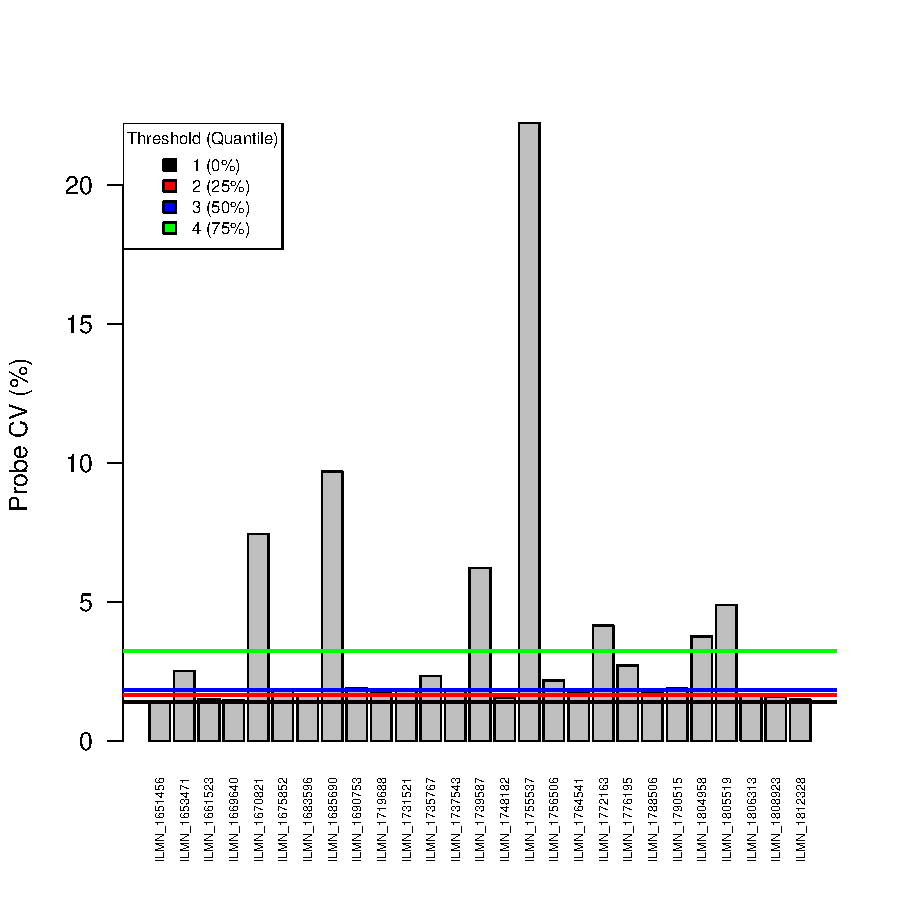
\includegraphics{massiR_Vignette-fig1}
\end{center}
\caption{Expression variation (CV) of Y chromosome probes across all samples}
\label{fig:fig1}
\end{figure}

\clearpage
After viewing the probe variation plot, a decision can be made regarding which probes to use in the clustering step. The massiR package includes methods for selecting probe variation thresholds based on quantiles. The threshold can be determined by quantiles of probe variance (CV): 1=All probes, 2=Upper 75\%, 3=Upper 50\%, 4=Upper 25\%. It is highly recommended that probe CV plot generated using the massi_y_plot function be inspected to inform threshold choice (Figure 1). The default threshold value is 3.

Once a probe threshold has been decided upon, run the massi.select function. This will return a data.frame with the samples as columns and the subset of selected y chromosome probes as row names.

\begin{Schunk}
\begin{Sinput}
> massi_select_out <- 
+   massi_select(massi.test.dataset, massi.test.probes, threshold=4)
\end{Sinput}
\end{Schunk}
Check the output for the first 5 samples:
\begin{Schunk}
\begin{Sinput}
> head(massi_select_out)[,1:5]
\end{Sinput}
\begin{Soutput}
                   S1       S2       S3       S4       S5
ILMN_1670821 5.746427 5.686032 6.307110 6.179258 6.594808
ILMN_1685690 5.459125 5.567289 6.919465 6.789817 6.559376
ILMN_1739587 5.883483 5.764190 6.441775 6.438789 6.707278
ILMN_1755537 5.882456 5.831844 8.133164 8.052959 8.298985
ILMN_1772163 5.696833 5.680091 5.907170 6.017871 6.465122
ILMN_1804958 5.815093 5.654395 5.929610 6.104089 5.868732
\end{Soutput}
\end{Schunk}

\section{Predicting the sex of samples}

To classify samples as either male or female, clustering is performed using the values from the subset of Y chromosome probes  by implementing the partitioning around medoids algorithm which performs k-medoids clustering (Hennig 2013), where samples are assigned to one of two clusters. The two clusters are then compared using the probe expression values across all samples in each cluster. Samples within the cluster featuring the highest Y chromosome probe values are classed as male and those within the cluster with the lowest Y probe values classed as female. Results such sample probe mean, standard deviation and z-scores are reported in a table together with the sex predicted for each sample.

To predict the sex of the samples using massi.cluster:
\begin{Schunk}
\begin{Sinput}
> results <- massi_cluster(massi_select_out)
\end{Sinput}
\end{Schunk}

Extract the results for each sample from the returned list:
\begin{Schunk}
\begin{Sinput}
> sample.results <- data.frame(results[[2]])
\end{Sinput}
\end{Schunk}

\begin{Schunk}
\begin{Sinput}
> head(sample.results)
\end{Sinput}
\begin{Soutput}
   ID mean_y_probes_value y_probes_sd    z_score    sex
1  S1            5.911089   0.4572756 -0.6453629 female
2 S10            6.749520   0.8418586  0.7773050   male
3 S11            5.689586   0.4750484 -1.1074329 female
4 S12            6.702993   0.7894613  0.7045705   male
5 S13            5.838450   0.6759924 -0.7193198 female
6 S14            5.819845   0.6593184 -0.7524047 female
\end{Soutput}
\end{Schunk}

As you can see, it is a relatively straightforward procedure to produce a table with the predicted sex of each sample with some basic metrics.

\section{Visualizing the massiR analysis data}

The massiR package includes a function which allows various aspects of the data used in the analysis to be visualized. These plots enable to used to inspect sample and clustering characteristics which could aid in identifying problematic samples and outliers.

To run the massi.plot function with the output from the massi.select and massi.cluster functions:
\begin{Schunk}
\begin{Sinput}
> massi_cluster_plot(massi_select_out, results)
\end{Sinput}
\end{Schunk}
This will generate a bar plot of mean values and standard deviation from the subset of Y chromosome probes used in K-medoids clustering (Figure 2), with the bars colored with respect to predicted sex. This function also generates a heat map with dendrogram of Y chromosome probes as rows and individual samples in columns (Figure 3) and a principal component plot showing clusters (Figure 4). These plots can iad the user in identifying sample outliers or probes that may not be informative in the clustering step. 

\clearpage

\begin{figure}
\begin{center}
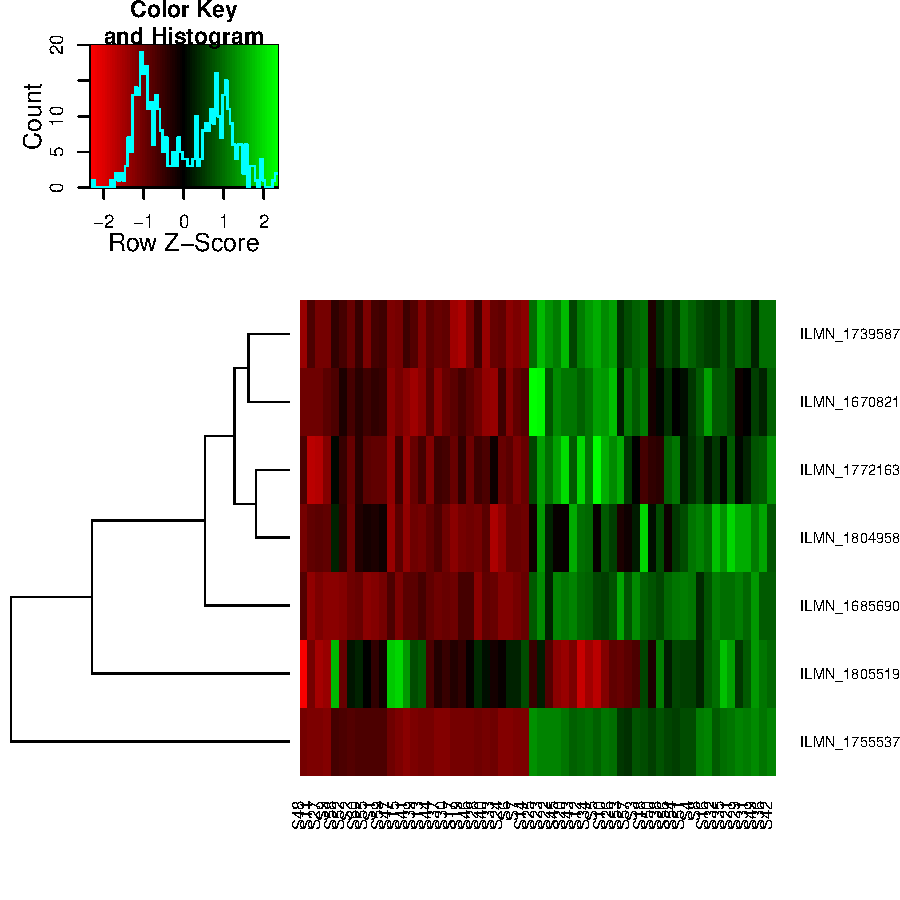
\includegraphics{massiR_Vignette-fig2}
\end{center}
\caption{Heat map with dendrogram of Y chromosome probes as rows and individual samples in columns. Notice that although the values for the probe in the fifth row are reasonably variable but do not show the same pattern seen with other probes. Therefore viewing the heatmap may help identify problematic probes.}
\label{fig:fig2}
\end{figure}

\begin{figure}
\begin{center}
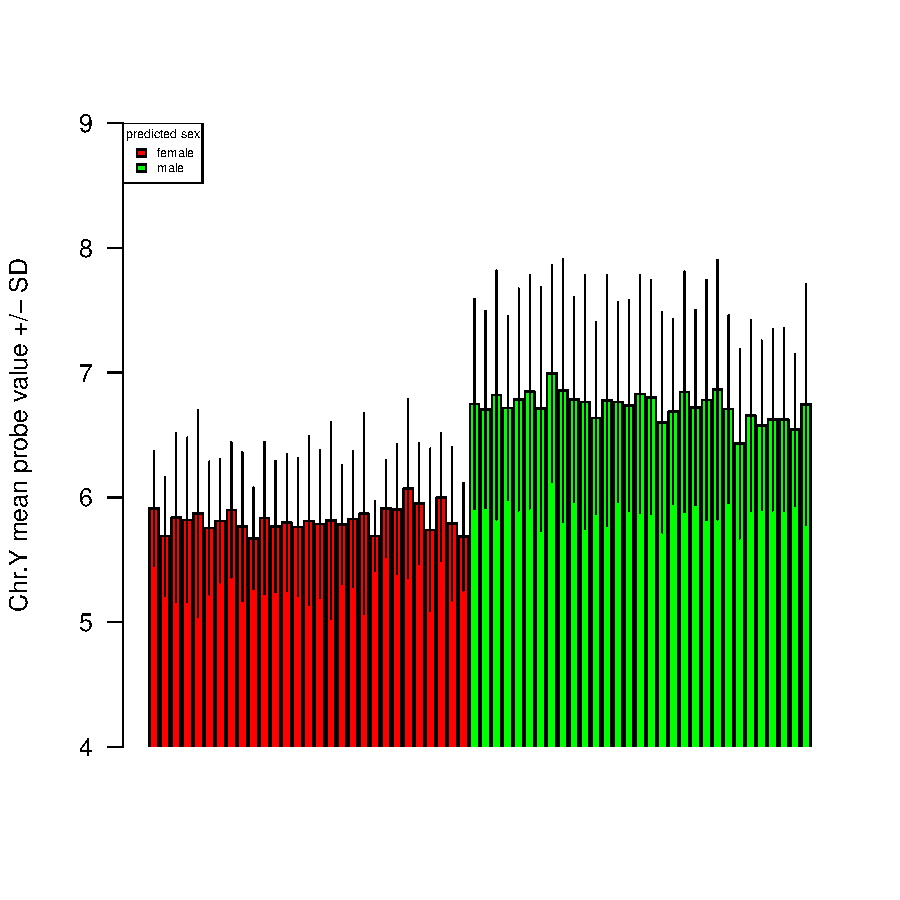
\includegraphics{massiR_Vignette-fig3}
\end{center}
\caption{Mean values of the subset of Y chromosome probes used in K-medoids clustering. The bar colors represent clusters, which were assigned as female (red) and male (green)}
\label{fig:fig3}
\end{figure}

\begin{figure}
\begin{center}
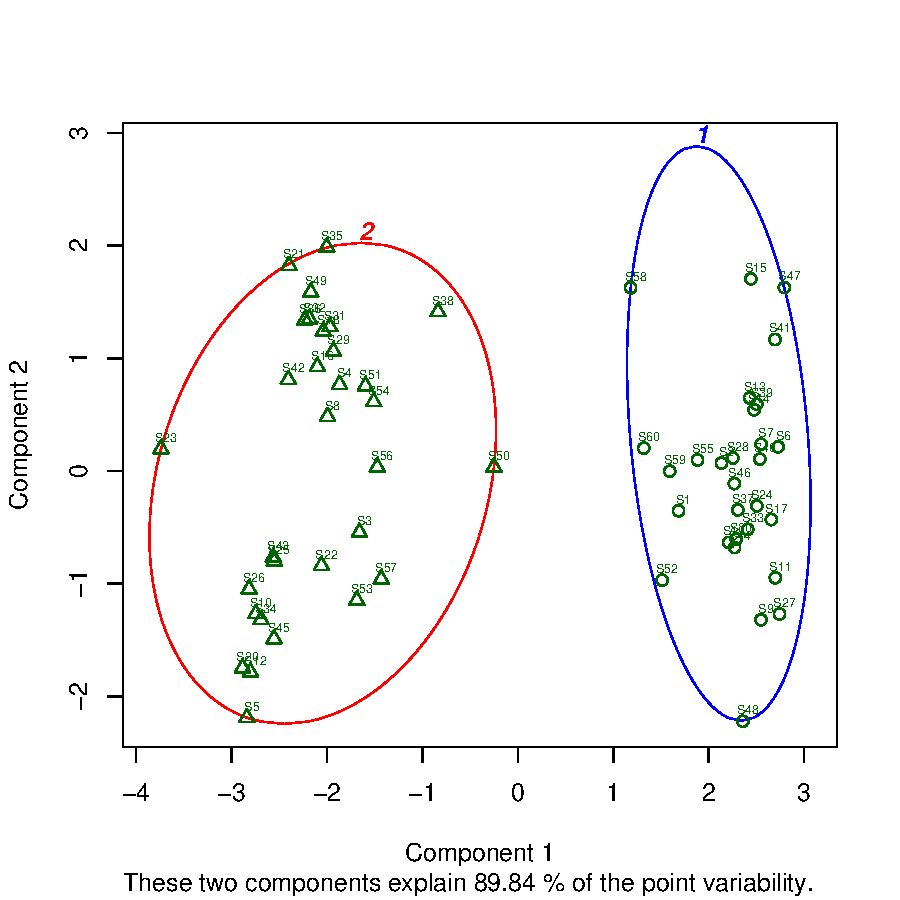
\includegraphics{massiR_Vignette-fig4}
\end{center}
\caption{Principal component plot of male and female clusters}
\label{fig:fig4}
\end{figure}

\clearpage

\section{Check for potential sex bias using the dip test}
The massiR method for predicting the sex of samples is >97\% accurate for data sets with 6 or more samples and with at least of 15\% of either males or females. Outside of this range, this method still performs well in most cases. As there is no guarantee that publicly available data sets will fall within these limits, the function massi.dip can be used to test if the data set might have a male/female ratio that might affect performance. 
\paragraph{} \hspace{0pt} \\
The massiR method was tested using empirical data sets for five different human tissues. Individual data subsets were randomly generated for each tissue data set ranging from 6-50 samples and with a wide-range of  Male/Female ratios. The results of this testing suggest for data sets with >10 samples a dip statistic  >0.08 is indicative of at least 15\% of males or females in the data set.

The massi.dip function calculates z-scores for each sample and implements the dip test to test for unimodality (Maechler 2013). As a relatively balanced dataset would typically show a bi-modal distribution of the z-scores, the dip statistic is then used to predict if a dataset shows a unimodal distribution that would  be expected if a vast majority of samples were of one sex.

To use massi_dip function, which calculates the dip statistic using the data output from the massi_select function:
\begin{Schunk}
\begin{Sinput}
> dip.result <- massi_dip(massi_select_out)
\end{Sinput}
\end{Schunk}

This returns the message:
{\color{red}dip test statistic is >0.08. This suggests that the proportion of male and female samples in this data set is relatively balanced}
\paragraph{} \hspace{0pt} \\

Visually inspecting this distribution as a density plot (figure 5) or a histogram plot (figure 6) enables the user to see if there is the expected bi-modal distribution  (as there should be distinct distributions for each sex).

To produce a density plot and histogram of sample z-scores:
\begin{figure}
\begin{center}
\begin{Schunk}
\begin{Sinput}
> dip.result <- massi_dip(massi_select_out)
> plot(dip.result[[3]])
\end{Sinput}
\end{Schunk}
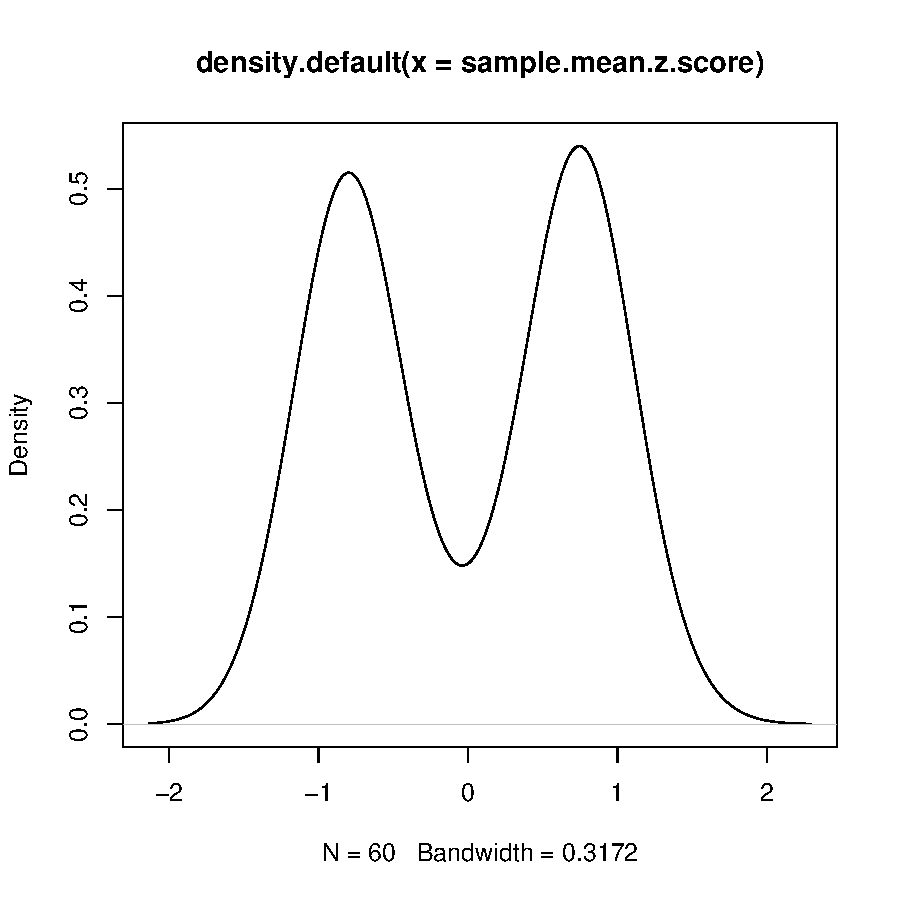
\includegraphics{massiR_Vignette-fig5}
\end{center}
\caption{Density plot of mean y chromosome probe z-scores}
\label{fig:fig5}
\end{figure}

\begin{figure}
\begin{center}
\begin{Schunk}
\begin{Sinput}
> dip.result <- massi_dip(massi_select_out)
> hist(x=dip.result[[2]], breaks=20)
\end{Sinput}
\end{Schunk}
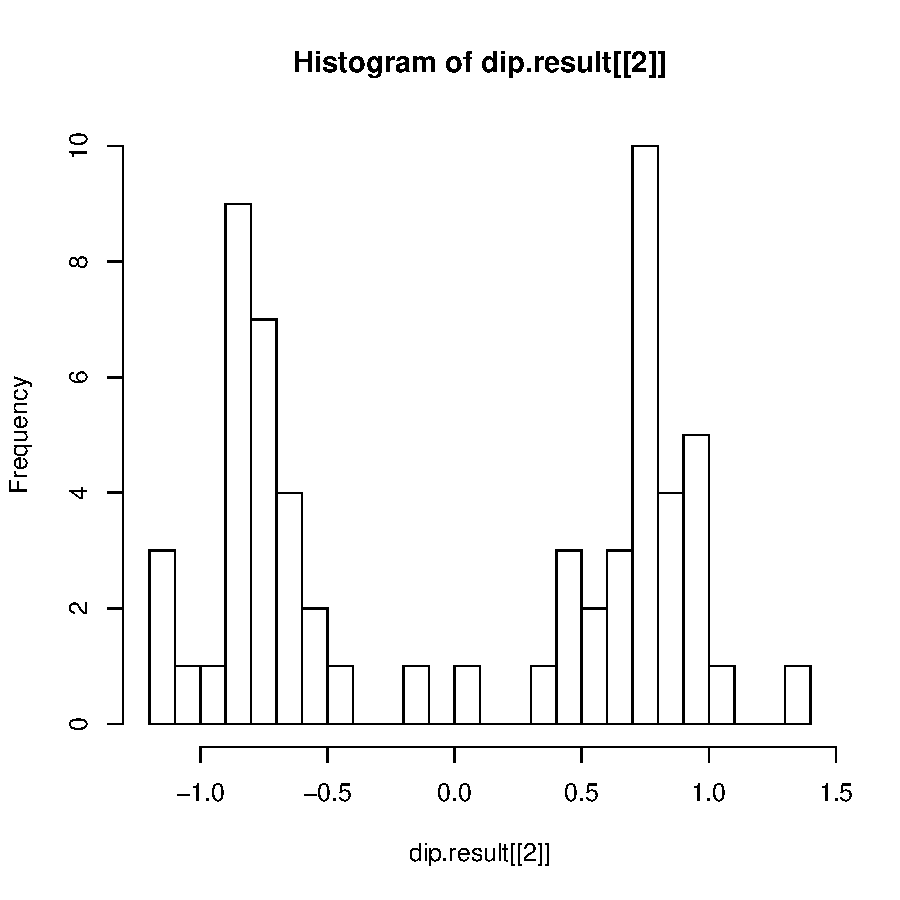
\includegraphics{massiR_Vignette-fig6}
\end{center}
\caption{Histogram of mean y chromosome probe z-scores}
\label{fig:fig6}
\end{figure}
\clearpage
If the data set was has a sex bias that may influence the accuracy of the massi sex prediction, then the massi.dip function is likely to return a dip statistic of <0.08. For example, if we are to use the massiR test data set to generate a subset to 20 samples composed of 10\% males, we will see that the dip statistic returned is <0.08.

To create this female skewed bias:

get the sample id's for the male and female samples:
\begin{Schunk}
\begin{Sinput}
> male.ids <-
+   subset(sample.results$ID,
+                    subset=sample.results$sex=="male")
> female.ids <-
+   subset(sample.results$ID,
+          subset=sample.results$sex=="female")
\end{Sinput}
\end{Schunk}
Create a data subsest of 20 samples with 10\% males:
\begin{Schunk}
\begin{Sinput}
> bias.subset.ids <- c(female.ids[1:18], male.ids[1:2])
> bias.subset <- massi_select_out[bias.subset.ids]
\end{Sinput}
\end{Schunk}
Use the massi.dip function to test for sex-biased data set:
\begin{Schunk}
\begin{Sinput}
> bias.dip <- massi_dip(bias.subset)
\end{Sinput}
\end{Schunk}

Please note that a dip >0.08 is a good indication that there is not a sex bias present that will affect the accuracy of the massiR method. However, and dip statistic <0.08 may still be returned for data sets with >15\% males or female or data sets that a suitable for massiR analysis, therefore the results of the massi.dip function should be interpreted with caution and in light of the massi.cluster results.

\section{Performing massiR analysis with an ExpressionSet object}

The massiR pipeline allows the input of expression data in the class ExpressionSet. 
Here is an example of how to use data in the ExpressionSet class in a massiR analysis and how to put the results back into the ExpressionSet:

Load the example ExpressionSet data included with the massiR package:
\begin{Schunk}
\begin{Sinput}
> data(massi.eset, massi.test.probes)
\end{Sinput}
\end{Schunk}

Using massiR with an ExpressionSet is the same as using a data.frame as in the above example:
\begin{Schunk}
\begin{Sinput}
> eset.select.out <- 
+   massi_select(massi.eset, massi.test.probes)
> eset.results <- 
+   massi_cluster(eset.select.out)
\end{Sinput}
\end{Schunk}

Now to get the massi.cluster results and add them to the ExpressionSet:
\begin{Schunk}
\begin{Sinput}
> # Get the sex for each sample from the massi.cluster results
> eset.sample.results <- 
+   data.frame(eset.results[[2]])
> sexData <- 
+   data.frame(eset.sample.results[c("ID", "sex")])
> # Exrtact the order of samples in the ExpressionSet and match with results
> eset.names <- 
+   colnames(exprs(massi.eset))
> # match the sample order in massiR results to the same as the ExpressionSet object
> sexData <- sexData[match(eset.names, sexData$ID),]
> # create an annotatedDataFrame to add to ExpressionSet
> pData <- new("AnnotatedDataFrame", data = sexData)
> # add the annotatedDataFrame to the Expressionset as phenoData
> phenoData(massi.eset) <- pData
\end{Sinput}
\end{Schunk}

Check the phenoData is in the ExpressionSet and double check that all sample id's from the massiR analysis match the sample identifiers in the ExpressionSet.

\begin{Schunk}
\begin{Sinput}
> # check the phenodata is now within the ExpressionSet
> phenoData(massi.eset)
\end{Sinput}
\begin{Soutput}
An object of class 'AnnotatedDataFrame'
  rowNames: 1 12 ... 57 (60 total)
  varLabels: ID sex
  varMetadata: labelDescription
\end{Soutput}
\end{Schunk}

\begin{Schunk}
\begin{Sinput}
> # check that all phenodata id's match expressionSet column names.
> # This must return "TRUE"
> all(massi.eset$ID == colnames(exprs(massi.eset)))
\end{Sinput}
\begin{Soutput}
[1] TRUE
\end{Soutput}
\end{Schunk}

\section{Using the included massiR y chromosome probe lists}

The massiR package includes lists of y chromosome probes for widely used Illumina and Affymetrix human gene expression platforms. 
If you wish to use one of the included probe lists, for example the Illumina human v2 probes:

Load the massiR included probe lists:
\begin{Schunk}
\begin{Sinput}
>  data(y.probes)
\end{Sinput}
\end{Schunk}
Check the names of the platforms for the probe lists.
\begin{Schunk}
\begin{Sinput}
>   names(y.probes)
\end{Sinput}
\begin{Soutput}
[1] "illumina_humanwg_6_v1" "illumina_humanwg_6_v2" "illumina_humanwg_6_v1"
[4] "illumina_humanht_12"   "affy_hugene_1_0_st_v1" "affy_hg_u133_plus_2"  
\end{Soutput}
\end{Schunk}
To get probe list into format for massiR analysis:
\begin{Schunk}
\begin{Sinput}
>   illumina.v2.probes <- data.frame(y.probes["illumina_humanwg_6_v2"])
\end{Sinput}
\end{Schunk}

The names of the probe lists correspond to Ensembl biomart attribute names.
For instructions on obtaining probe identifiers for other platforms, see the section "Using biomaRt to obtain y chromosome probe lists"

\section{Using biomaRt to obtain y chromosome probe lists}
Obtaining y chromosome probes lists for many microarray platforms is relatively easy using the biomaRt package (Durinik et al. 2005 and Durinik et al. 2009). This method is recommended because Ensembl have mapped probe sequences to reference genomes for many platforms and this allows ambiguous and non-specific probes to be removed. For details on probe mapping methods, see \url{<http://jan2013.archive.ensembl.org/info/docs/microarray_probe_set_mapping.html>}

For example, you can download the probes corresponding to the massiR test data set and obtain the Entrez gene id and genomic positions and convert these into a format for a massiR analysis:

Use the biomaRt package to download genomic regions and Entrez gene id's for Illumina v2 probes:
\begin{Schunk}
\begin{Sinput}
> library(biomaRt)
> mart <- useMart('ensembl', dataset="hsapiens_gene_ensembl")
> filters <- listFilters(mart)
> attributes <- listAttributes(mart)
> gene.attributes <- 
+  getBM(mart=mart, values=TRUE,
+        filters=c("with_illumina_humanwg_6_v2"),
+        attributes= c("illumina_humanwg_6_v2", "entrezgene",
+                       "chromosome_name", "start_position",
+                       "end_position", "strand"))
\end{Sinput}
\end{Schunk}
Remove the probes mapped to multiple genomic regions:
\begin{Schunk}
\begin{Sinput}
> unique.probe <- 
+   subset(gene.attributes, subset=!duplicated(gene.attributes[,1]))
\end{Sinput}
\end{Schunk}
Select the probes that correspond to y chromosome genes:
\begin{Schunk}
\begin{Sinput}
> y.unique <- 
+   subset(unique.probe, subset=unique.probe$chromosome_name == "Y")
\end{Sinput}
\end{Schunk}

Get the probe id's as row.names in the format for massiR analysis:
\begin{Schunk}
\begin{Sinput}
> illumina.v2.probes <- 
+   data.frame(row.names=y.unique$illumina_humanwg_6_v2)
\end{Sinput}
\end{Schunk}

This is a straightforwd way of obtaining Y chromosome probes for many microarray platforms that is independent of platform manufacturer annotations and is highly reccomended.

\clearpage

\section{References}
\paragraph{} \hspace{0pt} \\
  Christian Hennig (2013)
  fpc: Flexible procedures for clustering.
  R package version 2.1-6.
  http://CRAN.R-project.org/package=fpc
\paragraph{} \hspace{0pt} \\
  Martin Maechler (2013)
  diptest: Hartigan's dip test statistic for unimodality - corrected
  code. R package version 0.75-5.
  http://CRAN.R-project.org/package=diptest
\paragraph{} \hspace{0pt} \\
  Gregory R. Warnes, Ben Bolker, Lodewijk Bonebakker, Robert Gentleman,
  Wolfgang Huber, Andy Liaw, Thomas Lumley, Martin Maechler,
  Arni Magnusson, Steffen Moeller, Marc Schwartz and
  Bill Venables (2013).
  gplots: Various R programming tools for plotting data.
  R package version 2.12.1. http://CRAN.R-project.org/package=gplots
\paragraph{} \hspace{0pt} \\
  Steffen Durinck, Paul T. Spellman, Ewan Birney and Wolfgang Huber (2009)
  Mapping identifiers for the integration of genomic datasets
  with the R/Bioconductor package biomaRt.
  Nature Protocols 4, 1184-1191.
\paragraph{} \hspace{0pt} \\
  Steffen Durinck, Yves Moreau, Arek Kasprzyk, Sean Davis,
  Bart De Moor, Alvis Brazma and Wolfgang Huber (2005)
  BioMart and Bioconductor: a powerful link between biological databases
  and microarray data analysis.
  Bioinformatics 21, 3439-3440.
  
\end{document}
